
\section{Experiments} \label{sec:experiments}

We defined four workflow cases with different number of required activities based on the example of Section \ref{subsec:kb}. We performed experiments for measuring the size of the search space given the expected length of workflows. The length determines the size of the search space and thus the required time to perform the transformation. We used lengths from 6 to 14.

The growth of the search space is shown in Figure \ref{fig:graphs}. The size tends to be stable once it has reached the maximum length with all the required activities composed in sequence. For instance, $W1$ has $11$ required activities and it reaches the maximum length with $l=11$. The workflows with the "maximum" number of parallel compositions are the ones with the small $l$. For instance with $l=7$, $W1$ has the maximum number of parallel compositions\footnote{See http://goo.gl/XKZuL and http://goo.gl/z4iu3 for examples of lengths 7 and 11.}.

%\tabsize{tab:size}{Search space growth respect to the plan length}

%\tabtime{tab:time}{Time for workflow transformations with different lengths}

\begin{figure*}
	\centering
		\begin{tabular}{lr}
				\subfloat[Search space]{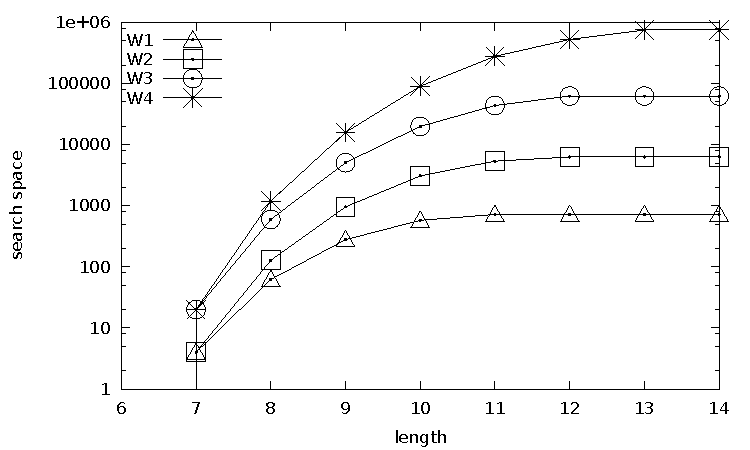
\epsfig{file=Images/searchspace.pdf, scale=0.47}\label{fig:searchspaceGraph}}
				&
				\subfloat[Execution time]{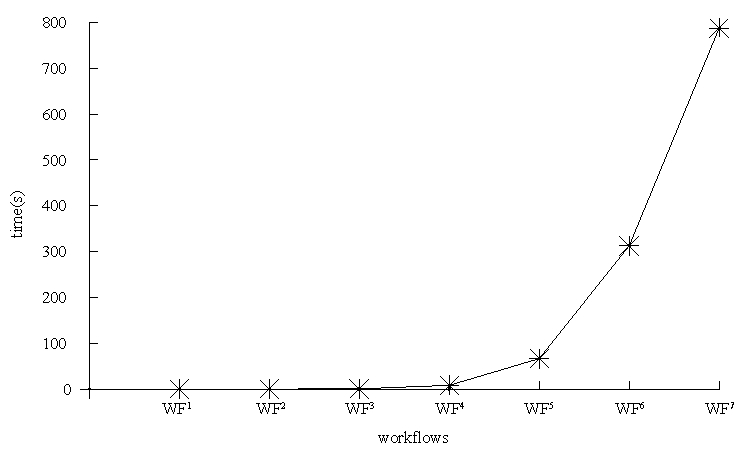
\epsfig{file=Images/time.pdf, scale=0.47}\label{fig:timeGraph}}			
		\end{tabular}
		\caption{Search space and execution time}
		\label{fig:graphs}
\end{figure*}

Besides the size of search space, the time for processing the workflow generation is exponential (\cf{} Figure \ref{fig:graphs}) and it is not feasible to generate completely the search space. Future work involves exploring alternative encodings and planning systems to obtain better performance.

